%% ----------------------------------------------------------------
%% Introduction.tex
%% ---------------------------------------------------------------- 
\chapter{Introduction} \label{Chapter:Introduction}
%The Introduction to my Report \dots

%The initial idea of the project was taken from Pirobot(\cite{Pirobot}).
%
%\inote{what it will do. Define everything. Use. Very general}
%General - mapping robots. 
%
%stereovision - uses etc.
%
%other similar projects
%
%why mine is important 

%\inote{Talk about what I set out to do, include some definitions etc. }
%\inote{What I ended up doing}
%\inote{The uses of my robot.} 


The original idea for the project was a stereoscopic mapping robot, similar to \cite{Pirobot}. This would autonomously search an area and return an occupancy map \citep{thrun2003learning}. The original project brief can be seen in Appendix \ref{Chapter:Appendix:Brief}. However, due to time constraints, the image processing aspects remain prototyped in \textsc{Matlab}, but not implemented in C. The end robot is able to capture stereo image pairs, move with reasonable accuracy and compute Fourier Transforms. The robot can run a predefined set of commands automatically or act as a shell terminal.

Stereoscopy in computer vision is the ability to calculate the locations and depths using images from two or more cameras, which are used to triangulate and estimate distances \citep{Saxena:DepthEstimation}. By using two cameras on the same plane, separated by a set horizontal distance, the depth of the observed scene can be perceived by the system.

Stereo vision is a small section of computer vision which is widely used in many applications. Microsoft's Xbox Kinect \citep{Microsoft:Kinect} uses stereo vision to locate a game player in order to use their movements to control the game. \cite{Mrovlje:Distance_Stereoscopic} used stereo vision to be able to locate the distance to a marker. 
\inote{Leap Motion?}

The stereo vision robot discussed in this report is a low cost alternative to other robots which use laser range finders or high quality cameras \citep{Se:MappingRobot}. The robot was mounted on the base seen in Figure \ref{fig:RobotBase} and used two OmniVision OV7670 cameras delivering colour QVGA format images.

The final robot could be used for a variety of applications. The robot can perceive depth of the captured area so can avoid obstacles and navigate. The robot could also be adapted to stream the camera data to a remote computer, and be controlled by a user to explore unknown and potentially hostile areas safely. 

\begin{figure}
\centering
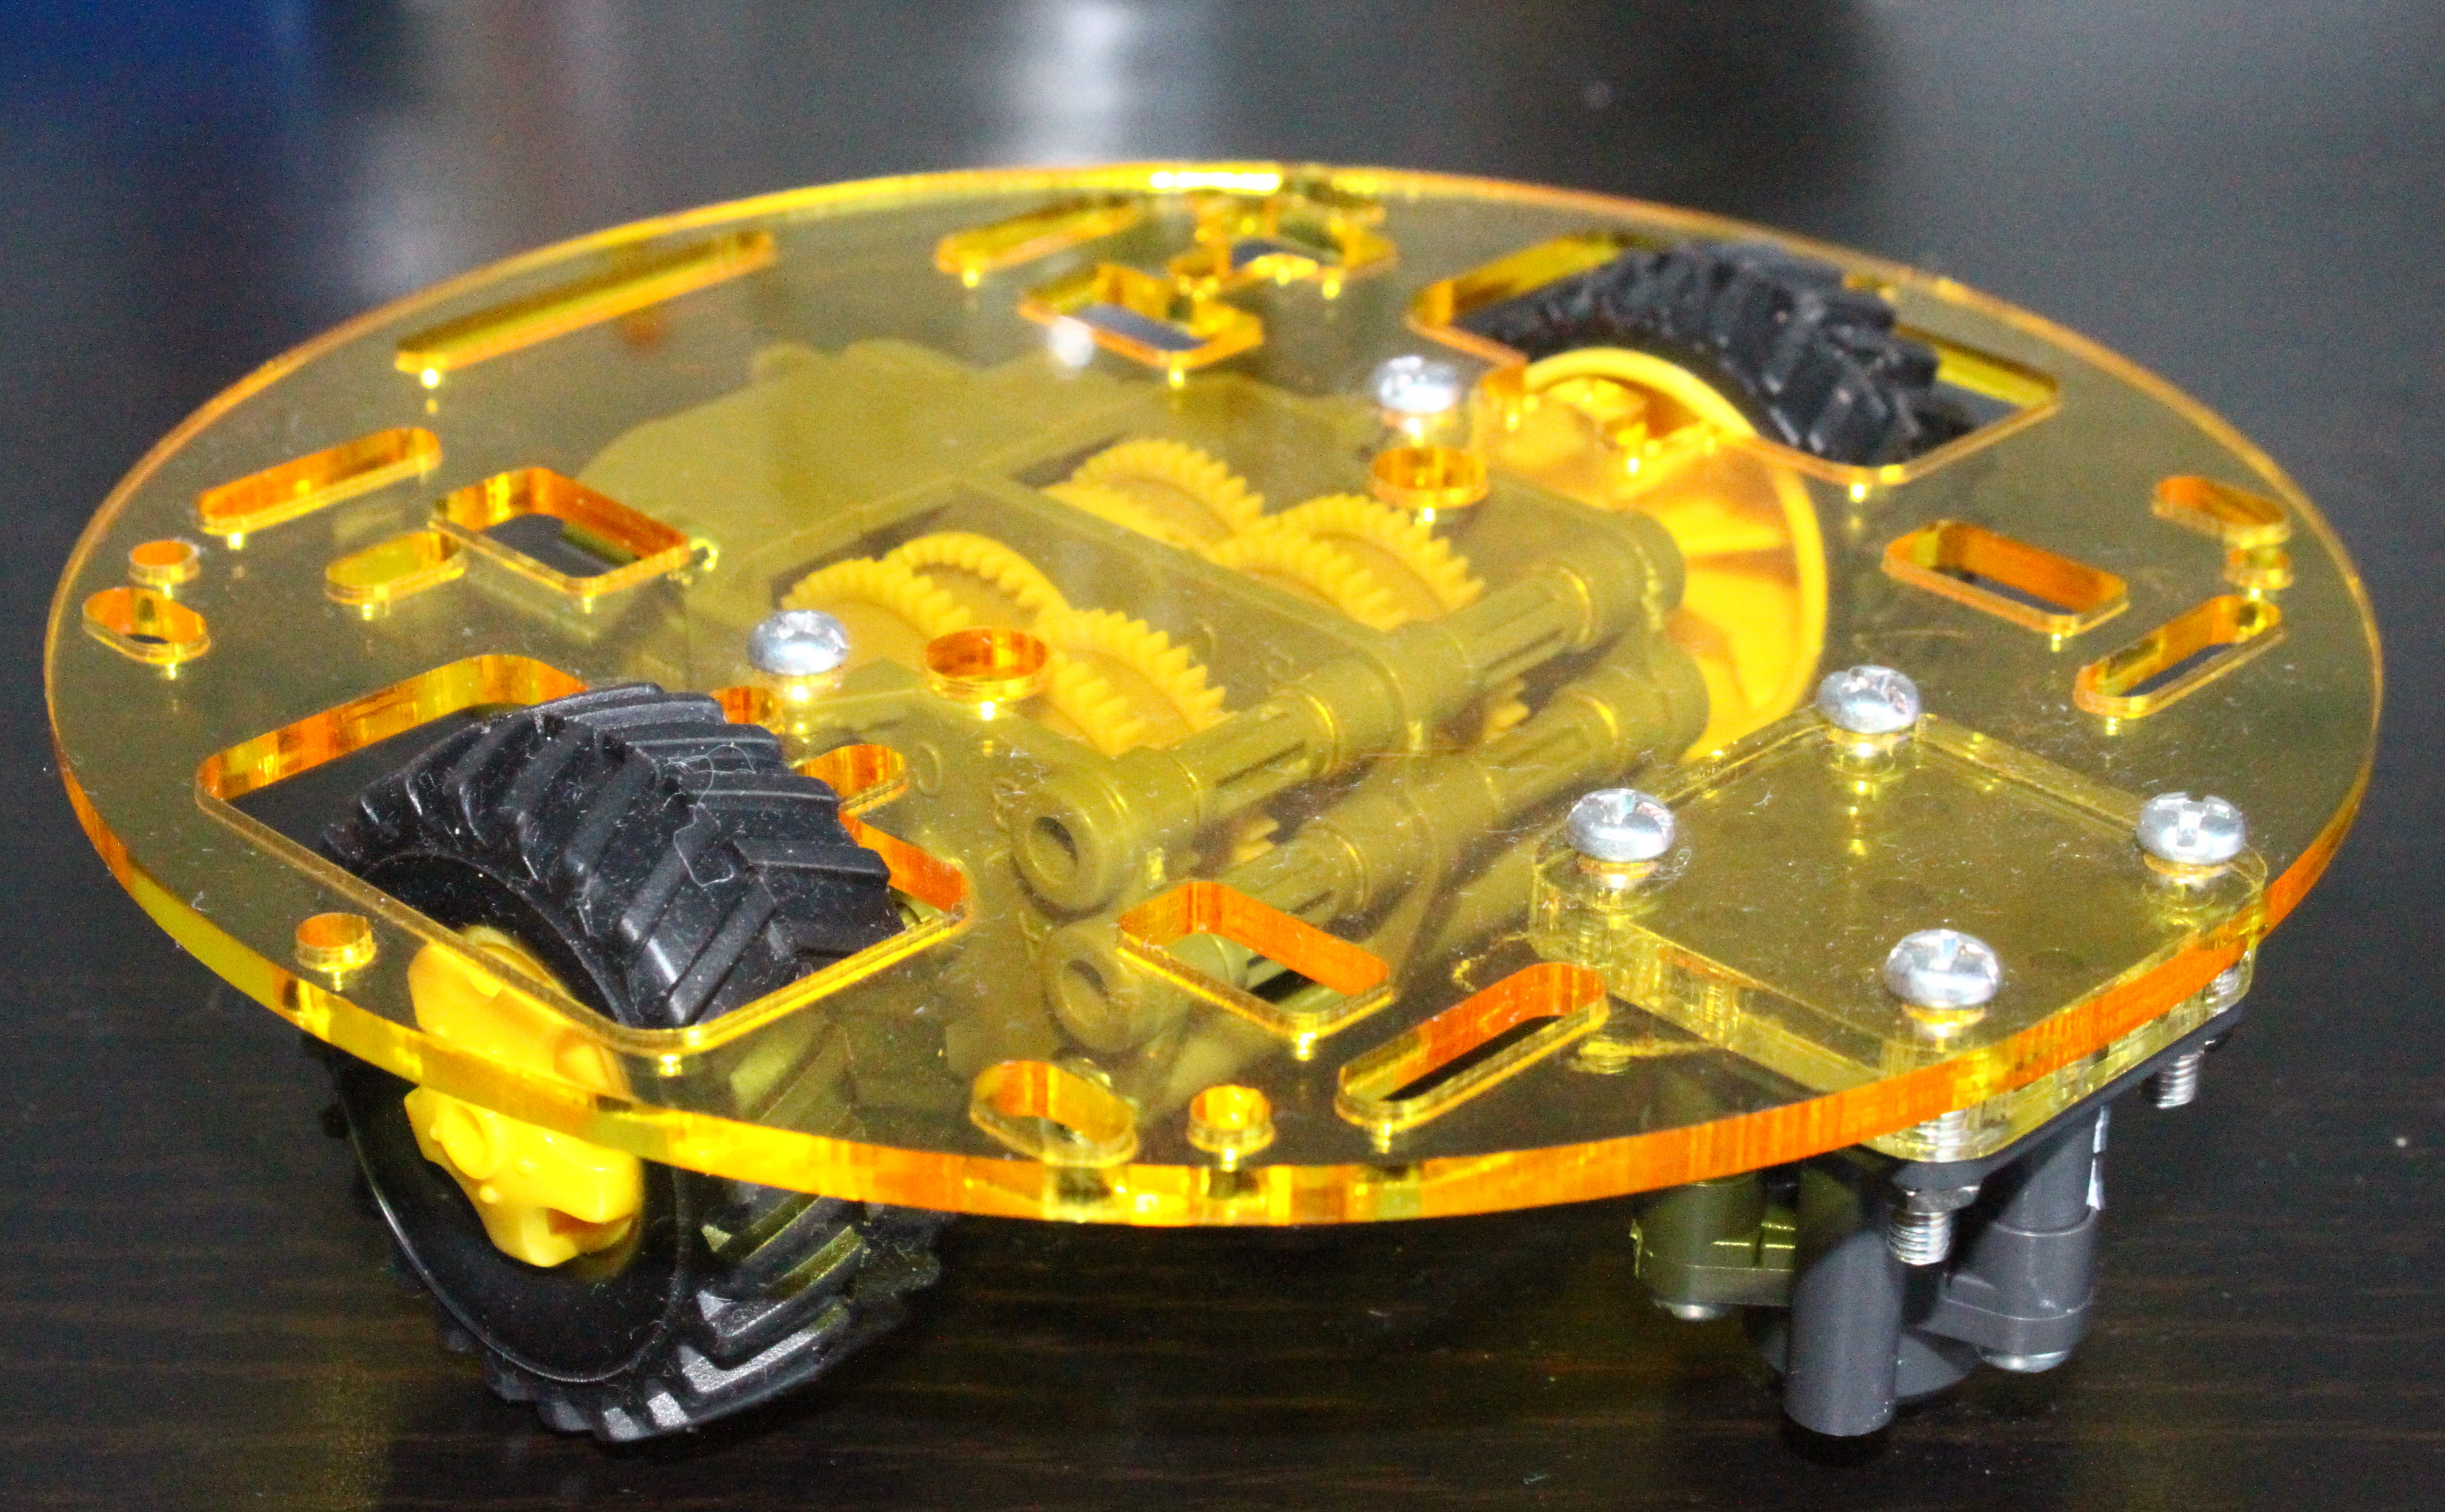
\includegraphics[width=\textwidth - 2cm]{./Figures/RobotBase.jpg}
\caption{The base of the robot}
\label{fig:RobotBase}
\end{figure}

\section{Project Management}
%In order to reduce the risk within the project, all aspects of potential issues were looked at and are summarised in table \ref{tab:risk}. A Gantt chart of how time was planned to be spent can be seen in figure \ref{fig:Gantt}.  

%The project was designed in stages - first, gaining operation of all the basic sections; movement, image capturing, image detection algorithms etc. These were then be brought together once tested to create the final product. This meant functionality was obtained of the basic aspects before addressing more complex issues. 

The project set ambitious targets. All sections of the design that needed addressing are seen in Table \ref{table:sections}. The project was developed using a spiral model to achieve the design aspects, starting with the hardware and firmware which were developed concurrently. This was done to obtain basic functionality first before concentrating on more complex aspects. Higher level algorithms were also prototyped during initial hardware development. However, the software was inherently dependent on the hardware. Therefore the hardware aspect was given priority. 

A number of risks were present during the project. These were assessed and steps were taken to reduce the chance of occurring. These can be seen in Table \ref{tab:risk}. 

At the beginning of the project, the Gantt chart in Figure \ref{fig:Gantt:1} was made. This was then reviewed after the interim report hand-in and anohter Gantt chart was made, seen in Figure \ref{fig:Gantt:2}, to show how time was allocated for the second semester. Figure \ref{fig:Gantt:3} documents how time was actually spent during the project. 

Figure \ref{fig:Gantt:3} shows that more time was spent on testing than originally anticipated. Also, while developing individual sections, small errors occurred that were time-consuming to correct, causing the time allocated to be insufficient. The motor driving required a large change when porting to the AT32, causing time to be spent developing this further. 

\begin{table}
\centering
\caption{Hardware and software aspects of the design}
\label{table:sections}
\begin{tabular}{cc}\toprule
\textbf{Hardware} & \textbf{Software} \\ \toprule
Single Camera	&	Firmware \\ \midrule
Dual Camera		&	Matching Algorithms \\ \midrule
SD Card			&	Range Finding \\ \midrule
Motor System	&	Mapping  \\ \midrule
PCB Design		&	Searching \\ \midrule
PCB Test		&	Testing \\ \bottomrule
\end{tabular}
\end{table}

\begin{table}
\centering
\caption{A list of risks and the prevention steps taken to reduce their impact}
\label{tab:risk}
\begin{tabular}{p{6cm}p{2cm}p{6cm}}\toprule
\textbf{Risk}						&	\textbf{Severity}	&	\textbf{Prevention} \\ \toprule
Components not arriving on time	&	High		&	Order parts as early as possible \\ \midrule
Project not fulfilling specification				&	High		&	Develop in stages to obtain functionality in parts. Ensure enough time is allocated to the project.	\\\midrule
PCB Design is incorrect		&	Medium		&	Check the design carefully and get second opinion. \\\midrule
Failure of personal computer causing data loss & Low	& 	Keep backups of all work on Devtrack Git repository and Dropbox.\\ \midrule
Damage to the robot through physical force or electrical connection & Medium & Ensure robot is transported in a box. Be careful not to connect the supply voltage to the $3V3$ rail to avoid damaging components. \\
\bottomrule
\end{tabular}
\end{table}

\section{Contributions}
The main part of this project was the hardware design and the embedded firmware development. \textsc{Matlab} skills had to be learnt for the prototyping of high-level algorithms for image processing. The skills obtained in \textsc{Matlab} also included producing graphs and 3D plots as well as general use of the software. Programming for a 32 bit Atmel microcontroller also had to be learnt during the project. This project supplied a practical use for theory learnt in lectures of the Fourier transform and cross correlation. 
